% !TeX document-id = {c68f4be8-c497-43e0-82df-e9ebfbea9577}
% !TeX TXS-program:pdflatex = pdflatex -synctex=1 -interaction=nonstopmode --shell-escape %.tex
% новая команда \RNumb для вывода римских цифр
\documentclass[a4paper,12pt]{article}
\usepackage{amssymb}
\usepackage{amsmath}
\usepackage{amsthm} 
\usepackage{caption}
\usepackage{misccorr}
\usepackage[noadjust]{cite}
\usepackage{cmap} 
\usepackage[utf8]{inputenc}
\usepackage[T2A]{fontenc}
\usepackage[english, russian]{babel}
\usepackage{graphics}
\usepackage{graphicx}
\usepackage{textcomp}
\usepackage{verbatim}
\usepackage{makeidx}
\usepackage{geometry}
\usepackage{float}
\usepackage{bm}
\usepackage{esint}
\usepackage{mathtools}
\usepackage{graphicx}
\usepackage{listings}
\usepackage{courier}
\usepackage{multirow}
\usepackage{graphicx}
\usepackage[table]{xcolor}
\usepackage{color}
\usepackage[most]{tcolorbox} 
\usepackage{diagbox}

\lstset{basicstyle=\fontsize{10}{10}\selectfont,breaklines=true}

\newcommand{\specchapter}[1]{\chapter*{#1}\addcontentsline{toc}{chapter}{#1}}
\newcommand{\specsection}[1]{\section*{#1}\addcontentsline{toc}{section}{#1}}
\newcommand{\specsubsection}[1]{\subsection*{#1}\addcontentsline{toc}{subsection}{#1}}
\newcommand{\RNumb}[1]{\uppercase\expandafter{\romannumeral #1\relax}}
\newcommand{\jj}{\righthyphenmin=20 \justifying}


% геометрия
\geometry{pdftex, left = 2cm, right = 2cm, top = 2.5cm, bottom = 2.5cm}

\setcounter{tocdepth}{4} % фикс переноса 
\righthyphenmin = 2
\tolerance = 2048

\begin{document}
	\thispagestyle{empty}
	
	\noindent \begin{minipage}{0.15\textwidth}
		
\includegraphics[width=\linewidth]{b_logo}
	\end{minipage}
	\noindent\begin{minipage}{0.9\textwidth}\centering
		\textbf{Министерство науки и высшего образования Российской Федерации}\\
		\textbf{Федеральное государственное бюджетное образовательное учреждение высшего образования}\\
		\textbf{«Московский государственный технический университет имени Н.Э.~Баумана}\\
		\textbf{(национальный исследовательский университет)»}\\
		\textbf{(МГТУ им. Н.Э.~Баумана)}
	\end{minipage}
	
	\noindent\rule{18cm}{3pt}
	\newline\newline
	\noindent ФАКУЛЬТЕТ $\underline{\text{«Информатика и системы управления»}}$ \newline\newline
	\noindent КАФЕДРА $\underline{\text{«Компьютерные системы и сети»}}$\newline\newline
	\noindent НАПРАВЛЕНИЕ ПОДГОТОВКИ $\underline{\text{«09.03.04 Программная инженерия»}}$\newline\newline\newline\newline\newline
	
	
	\begin{center}
		\noindent\begin{minipage}{1.3\textwidth}\centering
			\Large\textbf{  РУБЕЖНЫЙ КОНТРОЛЬ №2 }\newline
			\textbf{<<Обобщенная схема последовательного ЗУ.}\newline
			\textbf{Стек и буфер FIFO>>}\newline\newline\newline\newline
		\end{minipage}
	\end{center}
	
	\begin{center}
		\begin{tabular}{ccccc}
			Студент: & $\underline{\text{ИУ7-43Б}}$ & $\underline{\text{~~~~~~~~~~~}}$ & $\underline{\text{02.05.2020}}$ & $\underline{\text{А. В. Романов}}$ \\
			& \footnotesize группа & \footnotesize подпись & \footnotesize дата  & \footnotesize (И. О. Фамилия) \\
			&  &  &  & \\
			Преподаватель: & \textbf{} & $\underline{\text{~~~~~~~~~~~}}$ & $\underline{\text{~~~~~~~~~~~~}}$ & $\underline{\text{А. Ю. Попов}}$ \\
			&  & \footnotesize подпись & \footnotesize дата  & \footnotesize (И. О. Фамилия) \\
		\end{tabular}
	\end{center}
	
	
	\begin{center}
		\vfill
		Москва~---~\the\year
		~г.
	\end{center}
	\clearpage
	
	\noindent Последовательные ЗУ - так же как и другие, пишутся и читаются. Обычно используются в том случае, если данные могут быть выстроены в очередь, \newline
	
	\begin{center}
		\noindent 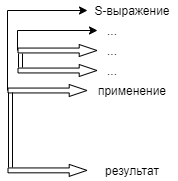
\includegraphics[scale=0.4]{1.png}\newline
	\end{center}
	
	\noindent \textbf{Стек} - LIFO (Last In, First Out). Стек - это абстракция. Реализовать вершину стека всегда возможно реализовать аппаратно. Может использоваться в арифметических операциях (польская запись). Обычно реализуют (как и буфер) на адресной памяти. \newline
	
	\noindent Пример реализации: сдвиг. Счётчик в данном случае реверсивный. В реализации стека можно 
	чтобы стек рос с конца, а можно и наооборот, это уже выбирается внутри устройства. То, есть, реализация полностью за нами, можно например по коду Грея (такой даже будет работать быстрее чем двоичный). Самый быстрый способ реализации: бегущая единица.
	
	\begin{center}
		\noindent 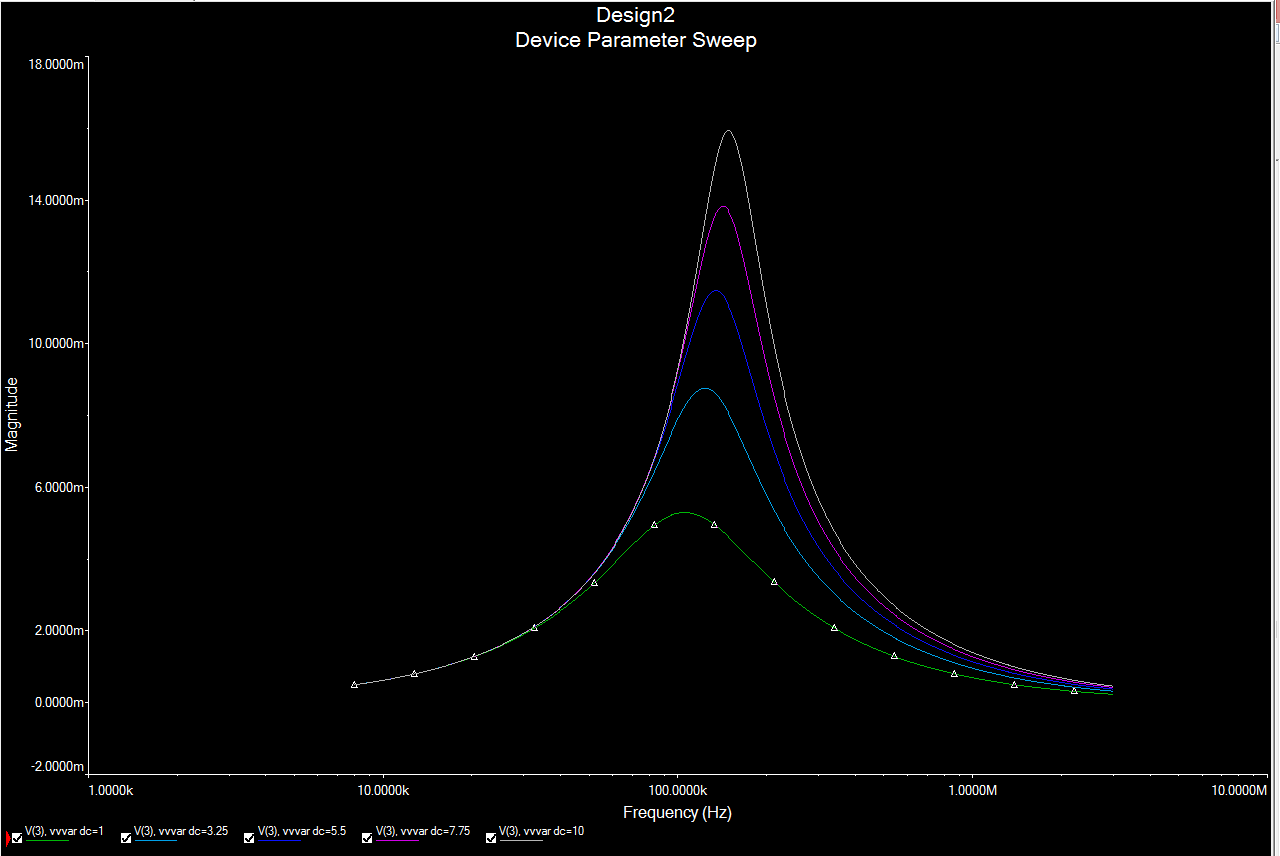
\includegraphics[scale=0.4]{2.png}\newline
	\end{center}

	\noindent \textbf{Буфер} - память реализованая как FIFO (First In, First Out). Помогает накапливать информацию. Важно накапливать данные - например если операция быстро выполняется, чтобы она не простаивала. Буфер FIFO решает проблему, когда оба конвейера готовы (один принять, другой передать).Но, важно понимать, что любой буфер плох для латентности (пока положим в буфер, достанем и тд, увеличивается время прохода.)\newline
	
	\noindent Об устройстве: есть запоминающий массив. Голову передаем следующей ступени, в хвост записываем. То есть нужны два адреса (головы и хвоста). При чтении и записи, понятное дело, нужно двигать указатели. Код операции выдается на мультиплексор (трапеция на фото), и она выбирает тот адрес, который нужно использовать (хвост или голову). На фото одно шина, но обычно используют две. Одна для чтения, другая для записи.
	
\end{document}